\documentclass[crop,border=7pt]{standalone}
\usepackage{tikz}
\usetikzlibrary{calc,patterns}
\begin{document}
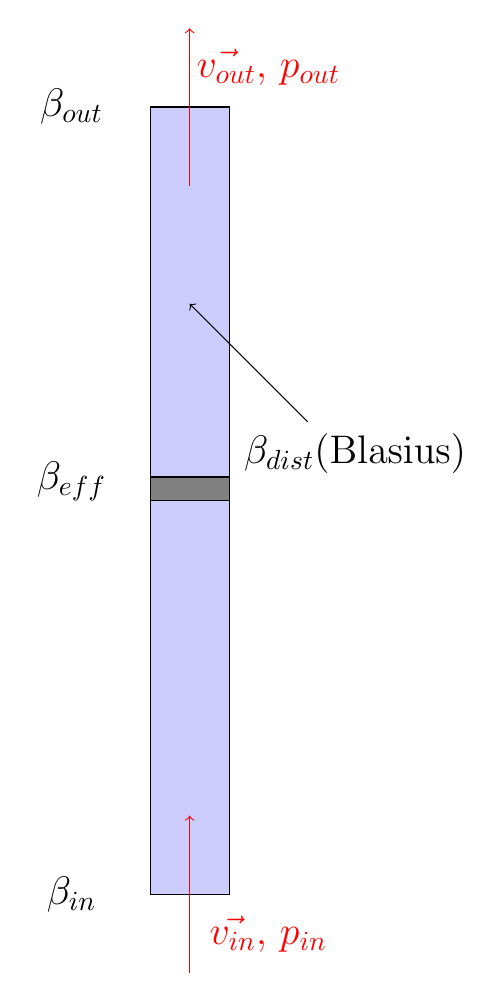
\begin{tikzpicture}

%%%%%%%%%%%%%%%%%%%%%%%%5

%PROFILE REACTOR
\filldraw[fill=blue!20, draw=black] (0,0) rectangle (1,10);
\draw [red, ->] (0.5,-1) -- (0.5,1);
\filldraw[fill=gray] (0,5) rectangle (1,5.3);
\node [align=right] at (1.5,-0.5) {\Large \textcolor{red}{$\vec{v_{in}}$, $p_{in}$}};
\draw [red, ->] (0.5,9) -- (0.5,11);
\node [align=right] at (1.5,10.5) {\Large \textcolor{red}{$\vec{v_{out}}$, $p_{out}$}};

\node [align=left] at (-1,0) {\Large \textbf{$\beta_{in}$}};
\node [align=left] at (-1,10) {\Large \textbf{$\beta_{out}$}};
\node [align=left] at (-1,5.25) {\Large \textbf{$\beta_{eff}$}};
%\draw (0,0) -- (4,0);

\draw [->] (2,6) -- (0.5,7.5);
\node [align=right] at (2.6,5.6) {\Large \textbf{$\beta_{dist}$}(Blasius)};
%\shade[top color=yellow, bottom color=black] (0,0) rectangle (2,-1);
 %   \filldraw[fill=green!20!white, draw=green!40!black] (0,0) rectangle (2,1);
 %   \draw[pattern=north east lines,pattern color=red] (0,0) rectangle (1,3);
 %   \draw[pattern=north west lines,pattern color=blue] (0,0) rectangle (3,1);
%    \draw[pattern=vertical lines] (2,0) rectangle (5,1);
%    \draw[pattern=horizontal lines,pattern color=yellow] (2,0) rectangle (3,3);

\end{tikzpicture}
\end{document}